\chapter{Estado del arte}

En la última década ha surgido una nueva necesidad social de <<transporte inteligente>>. Debido al carácter más seguro, más ecológico y más eficiente de los vehículos eléctricos y los avances en nuevas tecnologías para la conducción autónoma, multitud de empresas privadas están poniendo el foco en el desarrollo de estas tecnologías para solventar el problema de la conducción autónoma.
Empresas como Tesla, Google e incluso FaceBook dan una solución bastante robusta a un problema muy complejo: la conducción autónoma. Este problema técnico consiste en que una máquina es capaz de circular por una vía, típicamente carreteras y autopistas, sin la intervención de un humano en ningún momento del trayecto respetando las normas de circulación y tomando continuamente decisiones ante situaciones de diversa índole. Para llevar a cabo esta tarea los vehículos autónomos deben estar provistos de sensores (cámaras, radar, LIDAR, etc.) cada vez más sofisticados que les permitan captar información de su entorno para alimentar algoritmos que son capaces de tomar decisiones. Este problema se aborda típicamente mediante técnicas de aprendizaje automático.

Debido al auge de esta nueva tecnología por el avance que supone, muchas compañías han decidido desarrollar algoritmos que aporten solución a este problema, lo que ha llevado a la creación de un estándar. El estándar en cuestión es el conocido como J3016, que fue elaborado por la Sociedad de Ingenieros Automotrices (SAE) \cite{sae} y que establece los niveles de conducción autónoma según la capacidad del vehículo.

\begin{itemize}
    \item \textbf{Nivel 0} No hay automatización de la conducción. Las tareas de conducción son realizadas en su totalidad por el conductor.
    \item \textbf{Nivel 1} Asistencia al conductor. El vehículo tiene algún sistema de automatización de la conducción, ya sea para el control de movimiento longitudinal o el movimiento lateral, pero no ambas cosas a la vez. El conductor realiza el resto de tareas de conducción.
    \item \textbf{Nivel 2} Automatización parcial. El vehículo es capaz de actuar de forma independiente dentro de escenarios controlados y en situaciones específicas de conducción. El conductor debe seguir prestando atención a lo que ocurre a su alrededor para evitar posibles riesgos.
    \item \textbf{Nivel 3} Automatización condicional. El coche conduce completamente solo y el conductor controla que todo funcione correctamente. El coche también puede ser conducido de forma habitual en cualquier momento.
    \item \textbf{Nivel 4} Alta autonomía. El sistema cuenta con los sistemas de automatización presentes en el nivel 3 y con sistemas de detección de objetos y eventos. Además es capa de responder ante ellos. El sistema de automatización de la conducción posee un sistema de respaldo para actuar en caso de fallo del sistema principal y poder conducir hasta una situación de riesgo mínimo.
    \item \textbf{Nivel 5} Autonomía total. El sistema cuenta con todos los beneficios del sistema de automatización del nivel 4. Sin embargo, en este caso el vehículo podría seguir conduciendo en todo momento o circunstancia.
\end{itemize}

Algunos ejemplos importantes de conducción autónoma son: el \textit{DARPA Grand Challenge} y el \textit{Urban Challenge}. El DARPA Grand Challenge, organizado en 2004 y 2005 en Estados Unidos, fue una carrera de vehículos autónomos que debían recorrer 120 kms. por el desierto de Nevada sin intervención humana y disponiendo únicamente de un listado de puntos de control entre el principio y el final del recorrido. El Urban Challenge, organizado en 2007, fue una carrera de vehículos autónomos en entornos urbanos en los que debían recorrer 96 km. en menos de 6 horas. Estas dos competiciones científicas mostraron la viabilidad técnica de construir coches que condujeran solos en entornos reales.

En la actualidad se están desarrollando sistemas que toman decisiones empleando una red neuronal profunda, la cual recibe información del entorno mediante diferentes sensores (cámaras, radar, LIDAR, etc.). A partir de los datos recogidos por los sensores la red predice unos valores de salida que serán los empleados para la conducción. Las decisiones tomadas por la red neuronal están determinadas por los datos empleados durante el entrenamiento de la misma. Por lo tanto, cuanto más representativo sea el conjunto de datos, mejor rendimiento se espera que tenga la red, ya que conocerá todas las posibles situaciones en las que pueda encontrarse un vehículo.

Las siguientes secciones describen algunos de las bases de datos más extendidas y usadas en la conducción autónoma, algunos modelos en redes neuronales exitosos en esta aplicación y algunos computadores especializados para el procesamiento de redes neuronales en tiempo real.

\section{Bases de datos para conducción autónoma}
\label{sec:datasets}

La tarea de la conducción autónoma requiere que el vehículo sea capaz de tomar decisiones en todo momento ante cualquier escenario posible en las vías por las que circula. Para ello, hace uso de la información proporcionada por los sensores a bordo. El sensor más común y que más información aporta a la tarea de la conducción son las cámaras, que es la base de las redes que se explicarán en la siguiente sección. Para controlar todos los posibles escenarios en los que un vehículo puede verse involucrado hace falta un conjunto de datos lo suficientemente grande y representativo de todas ellas, y es por esto que en los últimos años y debido al auge de esta tecnología han aparecido multitud de bases de datos que ayudan a solucionar este problema.
    
\subsection{Comma.ai}

La empresa de conducción autónoma Comma.ai creó en 2016 un conjunto de datos ~\cite{comma} que permite probar modelos para controlar un vehículo autónomo. El conjunto de datos consta de 11 videoclips grabados a 20 Hz de una cámara Point Grey colocada en el parabrisas de un Acura ILX 2016. El conjunto de datos es un archivo zip comprimido de 45 GB que consta de un total de 7.25 horas de datos de conducción. Los fotogramas de vídeo tienen un tamaño de 160x320 píxeles. Junto a los archivos de vídeo hay un conjunto de medidas de sensores donde se registran medidas como la velocidad, la aceleración, el ángulo de giro, la ubicación GPS y los ángulos del giroscopio.
Además registran las marcas temporales en las que se midieron todos estos datos a través de los sensores y las marcas temporales de los fotogramas de la cámara. Los datos de los sensores se capturan en bruto y los fotogramas de la cámara en archivos HDF5 para que sean fáciles de utilizar en el aprendizaje automático y el software de control.

\subsection{Udacity}

Inicialmente, Udacity  \cite{udacity-data} poseía 40 GB de datos públicos para facilitar que las personas fueran capaces de construir modelos competitivos sin acceso al tipo de datos de conducción que Tesla o Google poseen. Sin embargo, debido a que los modelos de aprendizaje profundo necesitan muchos datos, la compañía publicó 183 GB adicionales de datos de conducción.

El conjunto de datos de Udacity \cite{udacity-dataset} consta de 223 GB de datos. Se grabaron datos de más de 70 minutos de conducción en días soleados y nublados, repartidos en dos días en Mountain View (California). La variedad de imágenes aumenta la calidad de los resultados y proporciona a los investigadores datos realistas para poder trabajar, ya que este conjunto de datos representa mejor los desafíos de la conducción en el mundo real y las condiciones variables de la carretera que cualquier simulador. Los datos almacenados constan de latitud, longitud, marcha, freno, aceleración, ángulos de dirección y velocidad.

\subsection {NuScenes}

Este mismo año, se ha presentado una nueva base de datos multimodal a gran escala para la conducción autónoma denominada NuScenes \cite{nuscenes-dataset}. Esta base de datos se ha convertido en relevante al incluir información de toda una gama de sensores que incluye 5 radares, 1 lidar, 6 cámaras, IMU y GPS. NuTonomy scenes(NuScenes) tiene 7 veces más anotaciones y 100 veces más imágenes que el conjunto de datos de KITTI [REFERENCIA] que cubre 23 categorías incluyendo diferentes vehículos, tipos de peatones, dispositivos de movilidad y otros objetos.
Este conjunto de datos recopila 1000 escenas de conducción grabadas en Boston y Singapur, las cuales son ciudades conocidas por su gran densidad de tráfico y situaciones complejas en la conducción. Estas escenas duran 20 segundos y están seleccionadas manualmente para mostrar diversas y diferentes maniobras de conducción, situaciones en la circulación y comportamientos inesperados.
La mejora que aporta este conjunto de datos es que ofrece solución al desafío de que hay una falta de conjuntos de datos multimodales a gran escala que son críticos, ya que ningún sensor es suficiente por sí solo y los tipos de sensores requieren cierta armonización, cosa de la que adolecen el resto de bases de datos mencionadas.

Además, se ha promovido el primer reto de detección de nuScenes que se lanzó en abril de 2019. Los ganadores y los resultados de los desafíos se anunciarán en el taller sobre conducción autónoma (\textit{nuScenes 3D detection challenge} como parte de \textit{the Workshop on Autonomous Driving at CVPR 2019}.).

\section{Redes neuronales para conducción autónoma}
\label{sec:nets}

La conducción autónoma no es posible sin un algoritmo que tome decisiones. En esta sección se describirán diferentes arquitecturas de redes neuronales empleadas con éxito en la conducción autónoma.

\subsection{Redes neuronales convolucionales}

El aprendizaje de extremo a extremo para conducción autónoma se ha explorado desde finales de los años ochenta. \textit{The Autonomous Land Vehicle in a Neural Network} (ALVINN) \cite{alvinn}  se desarrolló para aprender ángulos de dirección a partir de una cámara y las medidas proporcionadas por un láser mediante una red neuronal con una sola capa oculta. Basados en esta idea de redes de extremo a extremo (dada una imagen o imágenes se predicen ángulos de dirección), existen múltiples aproximaciones \cite{road} \cite{end2end} \cite{interpretable} de las cuales veremos algunas a continuación.

Un buen ejemplo de red de extremo a extremo es la red PilotNet  \cite{end2end} \cite{explaining-end2end} creada por NVidia. En \cite{end2end} se describe dicha red con detalle. Es una red neuronal convolucional (CNN) que mapea píxeles en crudo de una sola cámara frontal a comandos de dirección directamente. El comando propuesto por la CNN se compara con el comando deseado para la imagen en concreto y los pesos de la red se van ajustando para aproximar una salida de la red a la salida deseada. El ajuste de pesos se realiza empleando \textit{back propagation}.

La red PilotNet (Figura \ref{fig.pilotnet})  consta de 9 capas, que incluyen una capa de normalización, 5 capas convolucionales y 3 capas densamente conexas. La imagen de entrada se divide en planos YUV y se alimenta a la red con ellos. Las capas convolucionales fueron diseñadas para realizar la extracción de características y fueron elegidas a través de experimentos que variaban las configuraciones de las capas. Las dos primeras capas convolucionales usaban un \textit{stride} de 2x2 y un \textit{kernel} de 5x5, mientras que las 3 últimas capas usaban un \textit{non-stride} y un kernel 3x3. Las 3 capas densamente conexas fueron diseñadas para funcionar como controlador de la dirección, pero no es posible saber exactamente qué partes de la red funcionan principalmente como extractor de características y cuáles sirven como controlador. El sistema aprende automáticamente las representaciones internas, como la detección de características útiles de la carretera.

El objetivo de \cite{explaining-end2end} es explicar lo que PilotNet aprende y cómo toma sus decisiones. Con este fin, se desarrolla un método para determinar qué elementos en la imagen de la carretera influyen más en la decisión de la detección de PilotNet. Se puede encontrar un informe detallado de su método de detección de saliencia en \cite{visual}.

\begin{figure}
\begin{center}
	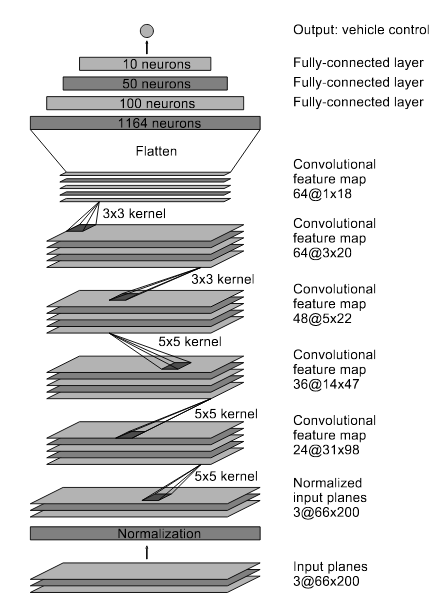
\includegraphics[width=0.3\textwidth]{img/pilotnet.png}
   \caption{Arquitectura Pilotnet.}
	\label{fig.pilotnet}
\end{center}
\end{figure}

La idea central de \cite{explaining-end2end} para discernir los objetos salientes es encontrar partes de la imagen que corresponden a ubicaciones donde los mapas de características tienen mejores activaciones. Las activaciones de los mapas de nivel superior se convierten en máscaras para las activaciones de niveles inferiores utilizando el siguiente algoritmo.

\begin{enumerate}
    \item En cada capa, las activaciones de los mapas de características se promedian.
    \item El mapa con el promedio más alto se escala según el tamaño del mapa de la capa de abajo. El aumento de escala se realiza mediante una de-convolución. Los parámetros (\textit{filter size y stride}) utilizados para la de-convolución son los mismos que se emplearon en la capa convolucional utilizada para generar el mapa. Los pesos de la de-convolución se establecen en 1.0 y los sesgos en 0.0.
    \item El mapa promediado aumentado de un nivel superior se multiplica después con el mapa promediado de la capa de abajo (ahora son del mismo tamaño). El resultado es una máscara de tamaño intermedio.
    \item La máscara intermedia se escala al tamaño de los mapas de la capa inferior de la misma manera que en el paso 2.
    \item El mapa intermedio mejorado se multiplica de nuevo con el mapa promediado de la capa de abajo. Se obtiene una nueva máscara intermedia.
    \item Los pasos 4 y 5 se repiten hasta que se alcanza la entrada. La última máscara que es del tamaño de la imagen de entrada se normaliza al rango 0-1 y se convierte en la máscara de visualización final.
\end{enumerate}

Esta máscara de visualización muestra qué regiones de la imagen de entrada contribuyen más a la salida de la red. Estas regiones identifican los objetos salientes. En la \ref{fig.salient} se pueden ver ejemplos de objetos salientes para varias imágenes de entrada.

\begin{figure}
\begin{center}
	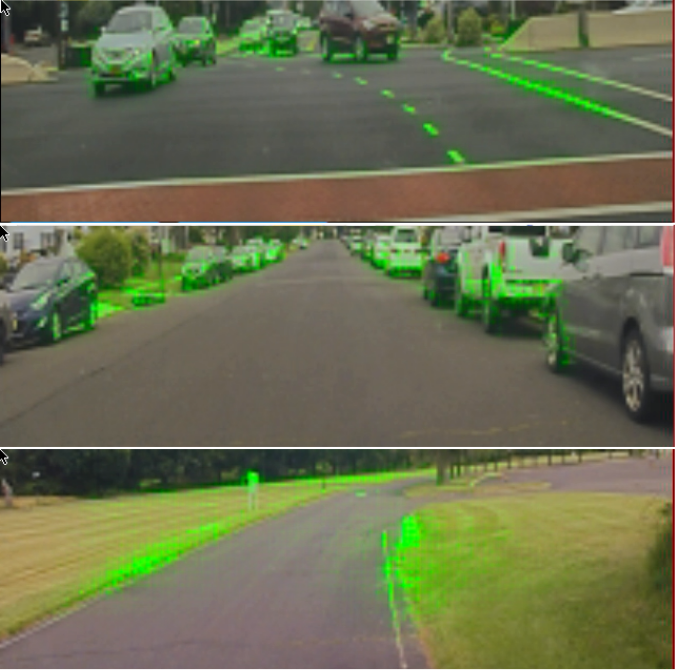
\includegraphics[width=0.4\textwidth]{img/saliencia.png}
   \caption{Ejemplos de objetos salientes para varias imágenes de entrada.}
	\label{fig.salient}
\end{center}
\end{figure}


Los resultados muestran que PilotNet aprende a reconocer objetos relevantes en la carretera y que es capaz de mantener el vehículo en el carril con éxito en una amplia variedad de condiciones, independientemente de si las marcas del carril están presentes en la carretera o no.

En \cite{self-driving} se propone una nueva arquitectura de red, llamada TinyPilotNet, que se deriva de la red PilotNet \cite{end2end} \cite{explaining-end2end}. La red TinyPilotNet (Figura \ref{fig.tinypilotnet}) está compuesta por una capa de entrada, en la que se introducirán imágenes de resolución 16x32 y un único canal, seguida por dos capas convolucionales de kernel 3x3, y una capa \textit{dropout} configurada al 50\% de probabilidad para agilizar el entrenamiento. Finalmente, el tensor de información se convierte en un vector que es conectado a dos capas densamente conexas que conducen a un par de neuronas, cada una de ellas dedicada a predecir los valores de dirección y aceleración respectivamente. La imagen de entrada tiene un solo canal formado por el canal de saturación del espacio de color HSV.

\begin{figure}
\begin{center}
	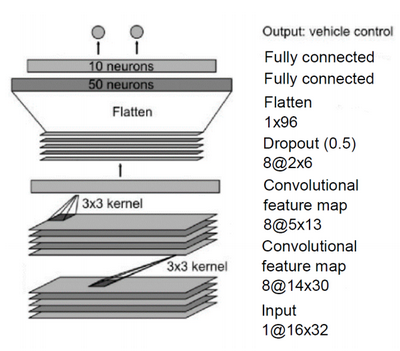
\includegraphics[width=0.5\textwidth]{img/tinypilotnet.png}
   \caption{Arquitectura TinyPilotnet.}
	\label{fig.tinypilotnet}
\end{center}
\end{figure}


En \cite{event} se presenta un enfoque de red neuronal profunda que emplea cámaras de eventos (sensores de inspiración biológica que no adquieren imágenes completas a una velocidad de fotogramas fija, sino que tiene píxeles independientes que solo producen cambios de intensidad de forma asíncrona en el momento en el que ocurren) para predecir el ángulo de giro de un vehículo. Los eventos se convierten en fotogramas de eventos por acumulación de píxeles en un intervalo de tiempo constante. Posteriormente, una red neuronal profunda los asigna a los ángulos de dirección.

En este artículo inicialmente apilan los fotogramas de eventos de diferente polaridad, creando una imagen de eventos 2D. Después, implementan una serie de arquitecturas ResNet, es decir ResNet18 y ResNet50. Estas redes son utilizadas como extractores de características para el problema de regresión, considerando sólo las capas convolucionales. Para codificar las características de la imagen extraídas de la última capa convolucional en un descriptor vectorizado, se emplea una capa \textit{global average pooling} que devuelve la media del canal de las características, Después se agrega una capa densamente conexa (con dimensionalidad 256 para ResNet18 y 1024 para ResNet50), seguida de una ReLu no lineal y una capa densamente conexa unidimensional para generar el ángulo.

En  \cite{event} predicen ángulos empleando 3 tipos de entradas: 1. imágenes en escala de grises, 2. diferencia de imágenes en escala de grises, 3. imágenes creadas por la acumulación de eventos. Analizan el rendimiento de la red en función del tiempo de integración utilizado para generar las imágenes de eventos (10, 25, 50, 100 y 200 ms). Cuanto mayor es el tiempo de integración, mayor es la traza de eventos que aparecen en los contornos de los objetos. La red funciona mejor cuando se entrena con imágenes de eventos correspondientes a 50 ms, y el rendimiento se degrada para tiempos de integración cada vez más grandes. Uno de los problemas que presentan las entradas que emplean imágenes en escala de grises es que a altas velocidades las imágenes se difuminan y la diferencia de imágenes se vuelve muy ruidosa.

En \cite{pixels} se realiza un amplio estudio donde se analiza una red neuronal de extremo a extremo para predecir las acciones de dirección de un vehículo en base a las imágenes de una cámara, así como las dependencias temporales de entradas consecutivas y la diferencia entre redes de clasificación y redes de regresión.

La arquitectura principal que emplean es una variación de la arquitectura PilotNet, AlexNet o VGG19. Para AlexNet se elimina el \textit{dropout} de las 2 capas densas finales y se reduce el tamaño de 500 a 200 neuronas. La capa de salida de la red depende de su tipo (regresión o clasificación) y para una red de clasificación del número de clases. Para el caso de clasificación, cuantifican las medidas del ángulo de dirección en valores discretos, que representan las etiquetas de la clase. Esta cuantificación es necesaria como entrada cuando se tiene una red de clasificación y permite equilibrar los datos a través de los pesos de la muestra. Esta ponderación actúa como un coeficiente para la tasa de aprendizaje de la red para cada muestra. El peso de una muestra está directamente relacionado con la clase a la que pertenece cuando se cuantifica. La ponderación de muestra se realiza para regresión y clasificación.

En este trabajo también se estudia la influencia de las especificaciones de cuantización de clase en el rendimiento del sistema. Estas especificaciones consisten en la cantidad de las clases y la asignación del rango de entrada de estas clases. Se comparan redes con diferentes grados de granularidad, lo que influye en el rendimiento. Se compara un esquema de cuantificación de grano grueso (son 7 clases) con uno de grano fino (17 clases), obteniendo mejores resultados con el de grano grueso. Además en este artículo se evalúan métodos que permiten que nuestro sistema aproveche la información de entradas consecutivas: un método que sigue una arquitectura de extremo a extremo y un método que emplea capas recurrentes (lo veremos en la siguiente subsección).

El método que emplea una CNN para la predicción, que llaman \textit{stacked frames}, concatena varias imágenes de entrada consecutivas para crear una imagen apilada. La entrada a la red es esta imagen apilada (para la imagen $t$ se concatenan las imágenes $t_1$, $t_2$, etc.). El tamaño de la entrada será la única variable que se modifique, es decir, no se modifica la red. Por esta razón, las imágenes se concatenan en la dimensión de profundidad (canal) y no en una nueva dimensión. Por ejemplo, apilar 2 imágenes anteriores a la imagen RGB actual de $160x320x3$ cambiaría su tamaño a $160x320x9$. Los resultados muestran un aumento en el rendimiento de las métricas con éste método. Se cree que es debido a que la red puede hacer una predicción basada en la información promedio de múltiples imágenes. Para una sola imagen, el valor predicho puede ser o muy alto o muy bajo. En cambio, para imágenes concatenadas, la información combinada podría cancelarse entre sí, dando una mejor predicción promedio. Suponiendo que la red promedie la información, aumentar el número de imágenes podría hacer que la red perdiera la capacidad de respuesta. Por ello emplean 3 fotogramas concatenados.

Además en este artículo se demuestra cualitativamente que las métricas estándar que se emplean para evaluar redes no necesariamente reflejan con precisión el comportamiento de conducción de un sistema. Una matriz de confusión prometedora puede dar como resultado un comportamiento de conducción deficiente, mientras que una matriz con mal aspecto puede dar como resultado un buen comportamiento de conducción.

\subsection{Redes neuronales recurrentes}

Las redes neuronales recurrentes (RNNs) representan una clase de redes neuronales artificiales que utilizan células de memoria para modelar la relación temporal entre los datos de entrada y, por lo tanto, aprender la dinámica subyacente. Con la introducción de las \textit{Long Short-Term Memory} (LSTM), el modelado de relaciones a largo plazo se hizo posible dentro de RNN.

En múltiples investigaciones sobre conducción autónoma se ha aprovechado la capacidad de estas redes para poder aprovechar la información de imágenes consecutivas, Algunas de estas investigaciones las veremos a continuación.

Un ejemplo de investigación donde se emplean capas LSTM es la propuesta por \cite{reactive-ground}. En esta investigación se presenta un controlador reactivo basado en aprendizaje profundo que emplea una arquitectura de red simple que requiere pocas imágenes de entrenamiento. A pesar de esta estructura simple, su arquitectura de red, llamada ControlNet, supera a otras redes más complejas en múltiples entornos (entornos interiores estructurados y entornos exteriores no estructurados) utilizando diferentes plataformas robóticas. Es decir, el artículo se centra en el control reactivo, donde el robot debe evitar obstáculos que no están presentes durante la construcción del mapa.

ControlNet extrae imágenes RGB para generar comandos de control: gira a la derecha, gira a la izquierda y recto. La arquitectura de ControlNet consiste en alternan capas convolucionales con capas de \textit{maxpooling} seguidas de capas densamente conexas. Las capas convolucionales y las de \textit{pooling} extra información geométrica sobre el medio ambiente, mientras que las capas densamente conexas actúan como un clasificador general. La capa LSTM permite al robot incorporar información temporal permitiéndole continuar moviéndose en la misma dirección sobre varios fotogramas. La estructura de ControlNet \ref{fig.controlnet}) es:

\begin{itemize}
    \item 2D Convolution, 16 filtros de tamaño 10x10
    \item Max Pooling, filtro de 3x3 stride de 2
    \item 2D Convolution, 16 filtros de tamaño 5x5
    \item Max Pooling, filtro de 3x3 stride de 2
    \item 2D Convolution, 16 filtros de tamaño 5x5
    \item Max Pooling, filtro de 3x3 stride de 2
    \item 2D Convolution, 16 filtros de tamaño 5x5
    \item Max Pooling, filtro de 3x3 stride de 2
    \item 2D Convolution, 16 filtros de tamaño 5x5
    \item Max Pooling, filtro de 3x3 stride de 2
    \item Fully connected, 50 neuronas
    \item ReLu
    \item Fully connected, 50 neuronas
    \item ReLu
    \item LSTM (5 frames)
    \item Softmax con 3 salidas
\end{itemize}

\begin{figure}
\begin{center}
	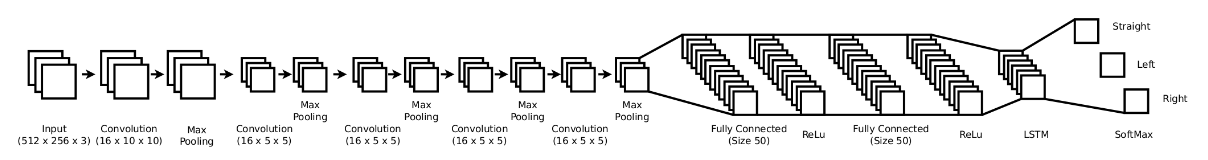
\includegraphics[width=1\textwidth]{img/controlnet.png}
   \caption{Estructura de red ControlNet.}
	\label{fig.controlnet}
\end{center}
\end{figure}

En \cite{temporal-dependencies} se propone una \textit{Convolutional Long Short-Term Memory Recurrent Neural Network}, conocido como C-LSTM (Figura \ref{fig.clstm}), que es entrenable de extremo a extremo, para aprender las dependencias visual y temporal dinámica de la conducción. El sistema investigado está compuesto por una cámara RGB frontal y una red neuronal que consta de una CNN y LSTM que estiman el ángulo del volante en función de la entrada de la cámara. Las imágenes de la cámara se procesan fotograma a fotograma por la CNN. Las características resultantes luego se procesan dentro de la red LSTM para aprender las dependencias temporales. La predicción del ángulo de dirección se calcula a través de la capa de clasificación de salida después de las capas LSTM.

Aplican el concepto de \textit{transfer learning}. La CNN está pre-entrenada en el conjunto de datos Imagenet. Luego, transfieren la red neuronal entrenada a otra específica enfocada en imágenes de conducción. Posteriormente, en la LSTM se procesa una secuencia de vectores de características de longitud fija $w$ de la CNN. A su vez, las capas LSTM aprenden a reconocer las dependencias temporales que conducen a una decisión de dirección $Y_t$ basada en las entradas de $X_{t-w}$ a $X_t$. Los valores pequeños de $t$ conducen a reacciones más rápidas, pero la red aprende solo las dependencias a corto plazo y la susceptibilidad a los aumentos de fotogramas mal clasificados individualmente. Mientras que los valores elevados de $t$ conducen a un comportamiento más suave y, por lo tanto, predicciones de dirección más estables, pero aumenta las posibilidades de aprender dependencias erróneas a largo plazo.

El concepto de ventana deslizante permite a la red aprender a reconocer diferentes ángulos de dirección desde el mismo fotograma $X_i$ pero en diferentes estados temporales de las capas LSTM. Tanto los pesos de la LSTM como de la CNN se comparten en diferentes pasos dentro de la ventana deslizante y, esto permite un tamaño de ventana arbitrariamente largo.

Plantean una regresión del ángulo de dirección como un problema de clasificación. Esta es la razón por la que el único número que representa el ángulo de dirección $Y_t$ está codificado como un vector de activaciones de las neuronas de la capa de clasificación. Utilizan una capa densamente conexa con activaciones $tanh$ para la capa de clasificación.

En esta propuesta para el entrenamiento de dominio "específico", la capa de clasificación de la CNN de reinicializa y se entrena con los datos de carretera de la cámara. El entrenamiento de la capa LSTM se lleva a cabo de manera múltiple, la red aprende las decisiones de dirección que están asociadas con los intervalos de conducción. La capa de clasificación y las capas LSTM emplean una mayor velocidad de aprendizaje porque se inicializan con valores aleatorios. La CNN y la LSTM se entrenan conjuntamente al mismo tiempo.

\begin{figure}
\begin{center}
	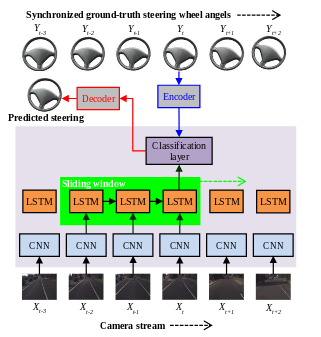
\includegraphics[width=0.5\textwidth]{img/clstm.png}
   \caption{Arquitectura C-LSTM.}
	\label{fig.clstm}
\end{center}
\end{figure}

En \cite{deep-steering} se propone un modelo basado en visión que mapea imágenes de entrada en ángulos de dirección usando redes profundas. Se segmenta la red en subredes. Es decir, los fotogramas se introducen primero en una red de extracción de características, generando una representación de características de longitud fija que modela el entorno visual y el estado interno de un vehículo. Las características extraídas se envían a una red de predicción de dirección. En la subred de extracción de características emplea una \textit{Spatio-Temporal Convolution} (ST-Conv) que cambia las dimensiones temporales y espaciales. Se emplea una capa densamente conexa tras la ST-Conv para obtener un vector de características de dimensión 128. Además, en la subred de extracción de características se introducen capas LSTM, para lo cual se emplea ConvLSTM. La subred de predicción de dirección propone concatenar acciones de dirección y de estado del vehículo con el vector de características de 128 dimensiones. Para ello se añade 1 paso de recurrencia entre la salida final y las dos capas \textit{concat} justo antes/después de la LSTM. La capa \textit{concat} antes de la LSTM agrega la velocidad, y el par de torsión y ángulo de rueda al vector de 128 dimensiones, formando un vector de 131 dimensiones. La capa \textit{concat} después de LSTM está compuesta por un vector de características 128-d + salida de LSTM 64-d + salida final previa 3d.

En \cite{interpretable} se propone un modelo de atención visual para entrenar una red convolucional de extremo a extremo desde las imágenes hasta el ángulo de giro. El modelo de atención resalta las regiones de imagen que potencialmente influyen en la salida de la red, de las cuales algunas son influencias reales y otras espúreas. Su modelo predice comandos de ángulo de dirección continuos a partir de píxeles en bruto. El modelo predice el radio de giro inverso $\hat{u}_t$, pero se relaciona con el comando de ángulo de dirección mediante geometría de Ackermann. 

En este método emplean una red neuronal convolucional para extraer un conjunto de vectores de características visuales codificadas, a las que se refieren como una característica convolucional cubo  $x_t$. Cada vector de características puede contener descripciones de objetos de alto nivel que permiten que el modelo de atención preste atención selectiva a ciertas partes de una imagen de entrada al elegir un subconjunto de vectores de características. Utilizan la red PilotNet \cite{end2end} para aprender un modelo de conducción, pero omiten las capas de \textit{maxpooling} para evitar la pérdida de información de ubicación espacial. Recopilan un cubo  $x_t$ de características convolucionales tridimensionales de la última capa empujando la imagen preprocesada a través del modelo, y el cubo de características de salida se emplea como entrada de las capas LSTM. Utilizan una red LSTM que predice el radio de giro inverso y genera ponderaciones de atención en cada paso de tiempo t condicionado al estado oculto anterior y una característica convolucional actual $x_t$. Asumen una capa oculta condicionada al estado oculto anterior y los vectores de características actuales. El peso de atención para cada ubicación espacial se calcula luego mediante una función de regresión logística multinomial.

El último paso de este método es un decodificador de grano fino en el que refinan un mapa de atención visual y detectan saliencias visuales locales. Aunque un mapa de atención del decodificador de grano grueso proporciona una probabilidad de importancia sobre un espacio de imagen 2D, el modelo debe determinar regiones específicas que causan un efecto casual en el rendimiento de la predicción. Obtienen una disminución en el rendimiento cuando se oculta una prominencia visual local en una imagen de entrada en bruto. En primer lugar, recopilan un conjunto consecutivo de pesos de atención e ingresan imágenes en bruto para los T pasos de  tiempo especificados por el usuario. Luego, crean un mapa de atención, $M_t$. La red neuronal de 5 capas (basada en PilotNet) emplea una pila de filtros 5x5 y 3x3 sin ninguna capa \textit{pooling}, y por tanto la imagen de dimensiones 80x160 se procesa para producir un cubo de características 10x20x64, conservando su relación de aspecto. Para extraer una prominencia visual local, primero muestrean aleatoriamente partículas de 2D con reemplazo sobre una imagen de entrada condicionada en el mapa de atención $M_t$. También emplean el eje de tiempo como la tercera dimensión para considerar las características temporales de las saliencias visuales, almacenando partículas espacio temporales 3D. Posteriormente, aplican un algoritmo de \textit{clustering} (DBSCAN) para encontrar una prominencia visual local agrupando las partículas 3D en \textit{clusters}. Para los puntos de cada grupo y cada fotograma de tiempo t, calculan el algoritmo \textit{convex hull} para encontrar una región local de cada prominencia visual destacada.

\begin{figure}
\begin{center}
	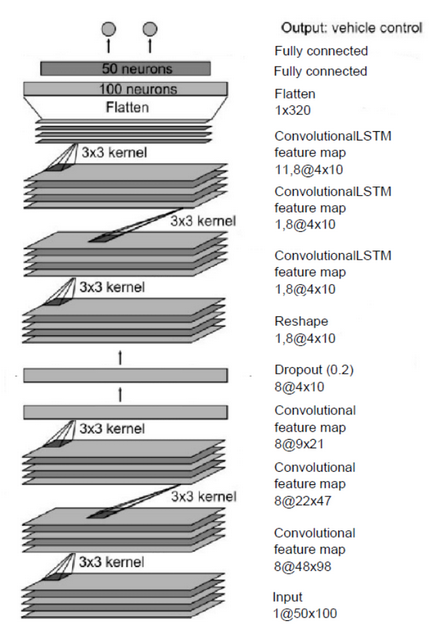
\includegraphics[width=0.4\textwidth]{img/deepestlstm.png}
   \caption{Arquitectura DeepestLSTM-TinyPilotnet.}
	\label{fig.deepestlstm}
\end{center}
\end{figure}

En \cite{pixels} además de aprovechar la información temporal concatenando fotogramas se estudia la inclusión de capas recurrentes. Es decir, modifican su arquitectura para incluir capas LSTM, que permiten capturar información temporal entre entradas consecutivas. Las redes se entrenan con un vector de entrada que consiste en la imagen de entrada y una serie de imágenes anteriores, lo que se traduce en una ventana de tiempo. Comparan muchas variaciones de la arquitectura PilotNet \cite{end2end}: (1) se cambia una o dos capas densas a capas LSTM, (2) se agrega una capa LSTM después de las capas densas, y (3) se cambia la capa de salida a LSTM. Todos los experimentos que realizan con redes LSTM demostraron que la incorporación de capas LSTM no aumentó ni redujo el rendimiento de la red.

En \cite{self-driving} se propone una nueva arquitectura basada en la arquitectura TinyPilotnet (Figura \ref{fig.tinypilotnet}) para mejorar el rendimiento de la misma. Esta nueva red (Figura \ref{fig.deepestlstm}) está formada principalmente por 3 capas convolucionales de kernel 3x3, combinadas con capas \textit{maxpooling}, seguidas por 3 capas LSTM convolucionales 5x5 y 2 capas densamente conexas. Las capas LSTM producen un efecto de memoria, por lo que los ángulos de dirección y los valores de aceleración dados por la CNN están influenciados por los anteriores. 

\section{\textit{Hardware} acelerador de cómputo neuronal}

Hasta ahora se han visto dos elementos esenciales del problema de la conducción autónoma mediante redes neuronales: las propias redes neuronales y los conjuntos de datos con los que se entrenan. Debido al carácter de los datos a procesar, donde se tiene información sensorial proveniente de cámaras (de color, de profundidad, de lineales, etc.) que ofrece una enorme cantidad de datos en cada imagen captada, es indispensable una alto poder computacional para procesar todos esos datos de forma eficiente y en tiempo real.

La conducción autónoma es una tarea donde el tiempo real es un aspecto crítico, ya que se trata un problema cuya solución ha abordarse desde una perspectiva de control híbrida (planificación + reacción) donde se requiere que la toma de decisiones por parte del algoritmo sea muy rápida para poder reaccionar de forma instantánea ante la gran cantidad de escenarios imprevistos que se pueden suceder durante la conducción (peatones que cruzan sin mirar, accidentes de tráfico, animales que cruzan la vía, etc.). No obstante, no todos los vehículos pueden estar dotados de computadores de grandes dimensiones como podría ser un computador de escritorio debido a las limitaciones tanto de alimentación como de espacio. Por este motivo, algunas empresas como Google o NVIDIA han creado \textit{hardware específico} para solventar este problema y ya no solo para aplicarlo a la conducción autónoma, sino también a cualquier problema domótico o, como tecnología en auge, IoT (\textit{Internet of Things}). 

En esta sección se describirán diferentes dispositivos diseñados para ser suficientemente potentes al ejecutar una red neuronal pesada y ocupar el mínimo espacio físico posible con el objetivo de empotrarlo en algún sistema.

\subsection{NVIDIA Jetson TK1}

En 2014, NVIDIA presentaba su primera placa para sistemas embebidos de alto rendimiento y bajo consumo, denominada Jetson TK1 \cite{jetsontk1}. Esta placa de dimensiones muy reducidas (127mm x 127mm) cuenta con un procesador ARM de 32-bits con 2 núcleos y una GPU con arquitectura Kepler que implementa 192 núcleos CUDA, ambos incluidos en el SoC (\textit{System-on-Chip}) Tegra K1 \cite{tegrak1}, además de una memoria RAM de 2 GB con tecnología DDR3. La presentación del procesador Tegra K1 fue un todo un hito, ya que fue el primer procesador móvil que igualaba en rendimiento a sistemas de escritorio con un bajísimo consumo de energía de $12.5\ W$ a máxima carga. 

\begin{figure}[htp]
    \centering
    \captionsetup{justification=centering}
    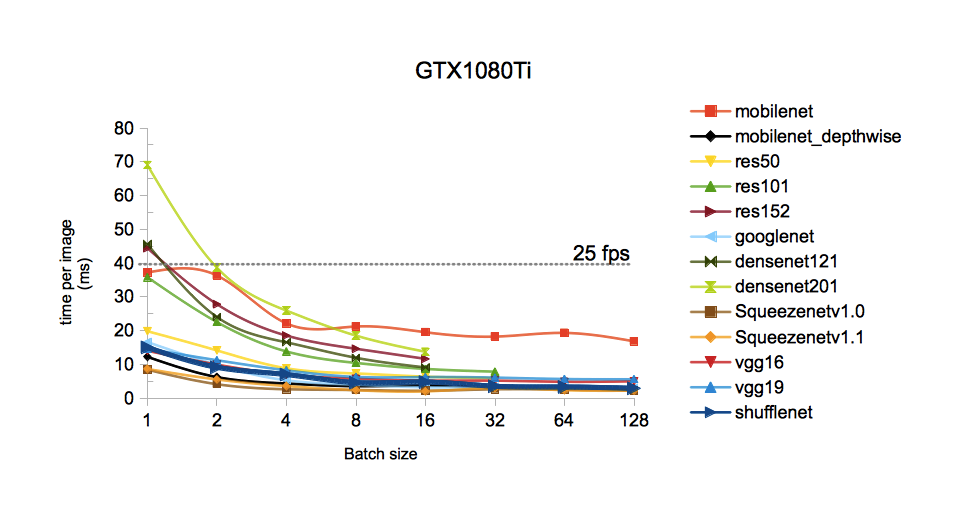
\includegraphics[width=.5\textwidth]{img/gtx1080_linear.png}\hfill
    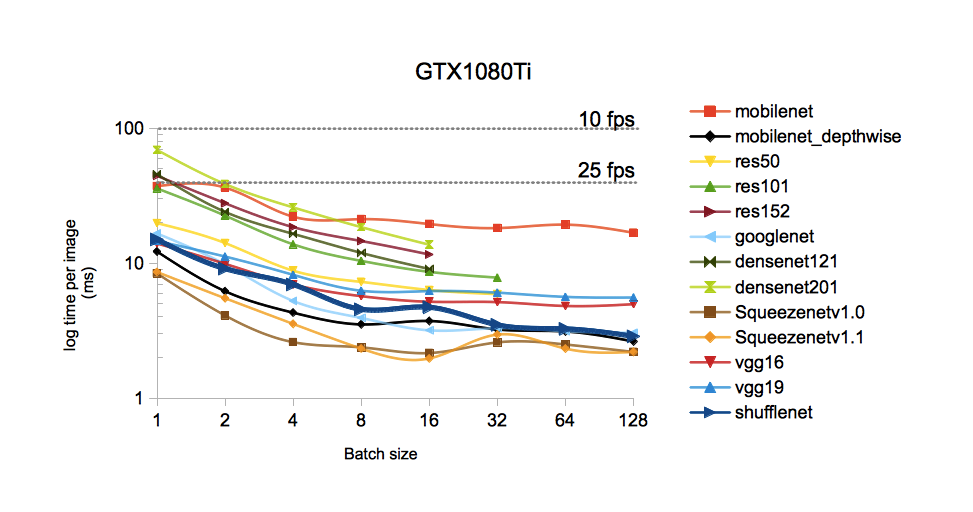
\includegraphics[width=.5\textwidth]{img/gtx1080_log.png}
    \caption{\textit{Benchmark} de referencia de la NVIDIA GTX 1080 de escritorio. (Izquierda) tiempo de procesamiento lineal. (Derecha) tiempo de procesamiento en escala logarítmica.}
    \label{fig:ben_gtx}
\end{figure}

\begin{figure}[htp]
    \centering
    \captionsetup{justification=centering}
    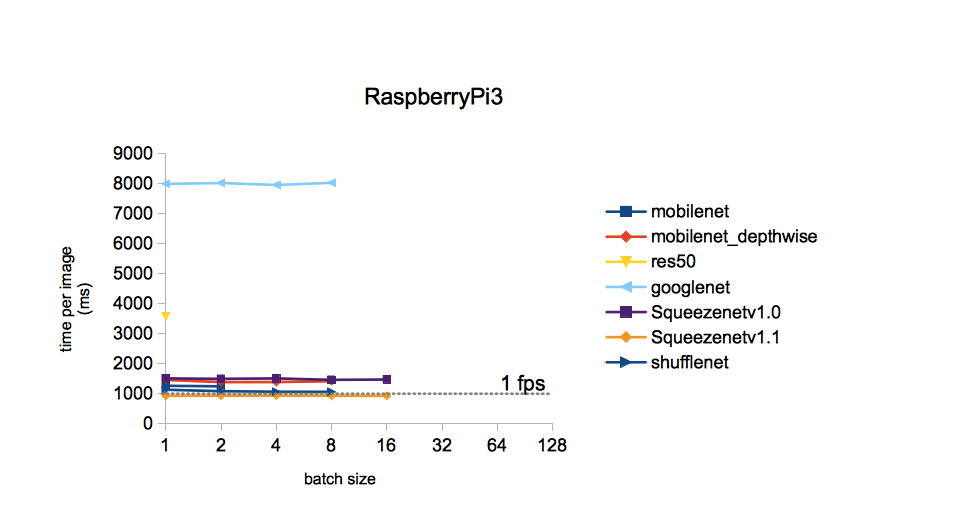
\includegraphics[width=.5\textwidth]{img/Raspi_linear.png}\hfill
    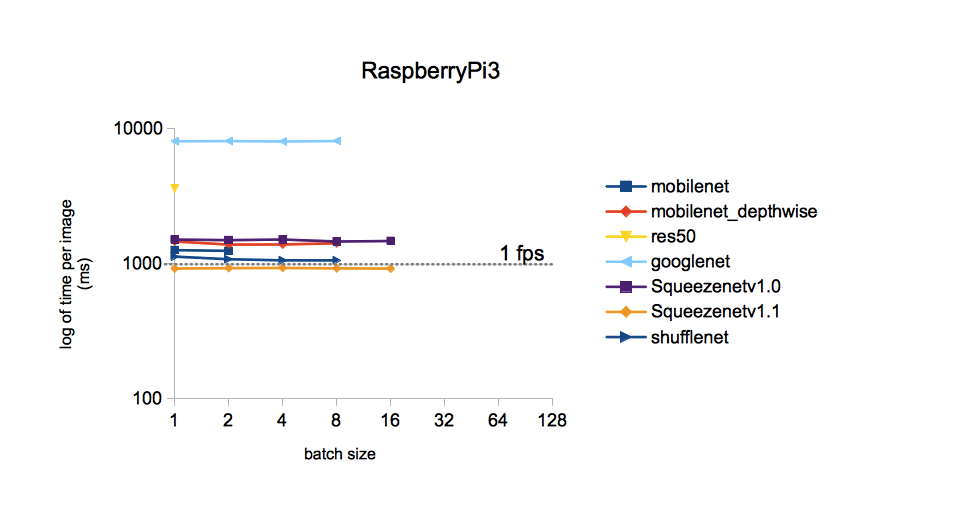
\includegraphics[width=.5\textwidth]{img/Raspi_log.png}
    \caption{\textit{Benchmark} de referencia de una Raspberry Pi3. (Izquierda) tiempo de procesamiento lineal. (Derecha) tiempo de procesamiento en escala logarítmica.}
    \label{fig:ben_pi}
\end{figure}

Se han realizado algunos \textit{Benchmarks} de esta placa probando su rendimiento con la ejecución de algunas redes neuronales modernas desarrolladas para sistemas embebidos, como \textit{mobilenet}, \textit{googlenet} o \textit{shufflenet} entre otras. Como referencia, en la Figura \ref{fig:ben_gtx} se tiene este mismo \textit{benchmark} medido sobre una tarjeta gráfica de alta gama para sistemas de escritorio, la NVIDIA GTX 1080Ti como referencia techo, y en la Figura \ref{fig:ben_pi} la referencia suelo de este mismo \textit{benchmark} llevado a una RaspberryPi modelo 3.

Los resultados se miden como la media de tiempo (en $ms$) que tarda el SoC TK1 en procesar una imagen frente a un tamaño de lote determinado de la red neuronal. Como se puede observar en la Figura \ref{fig:ben_tk1} (izquierda) la red más lenta es la \textit{mobilenet} con un tiempo de procesamiento por imagen de casi medio segundo ($500\ ms$), mientras que la red más rápida es la \textit{shufflenet v1.1} con un tiempo de procesamiento por debajo de los $100\ ms$, lo que aporta una tasa de fotogramas por segundo relevante. En la Figura \ref{fig:ben_tk1} (derecha) se puede apreciar con mayor claridad el rendimiento de esta placa con diferentes redes neuronales.

No obstante, si se compara esta placa con una RaspberryPi 3, los resultados son significativos, ya que su rendimiento es más del doble con respecto a la Raspberry. Y si se compara por arriba con la GTX 1080, no está muy lejos de los mínimos de esta, por lo que el poder computacional con respecto a la energía consumida es notable. Todo esto se puede ver reflejado en la Figura \ref{fig:ben_tk1_comp}

\begin{figure}[htp]
    \centering
    \captionsetup{justification=centering}
    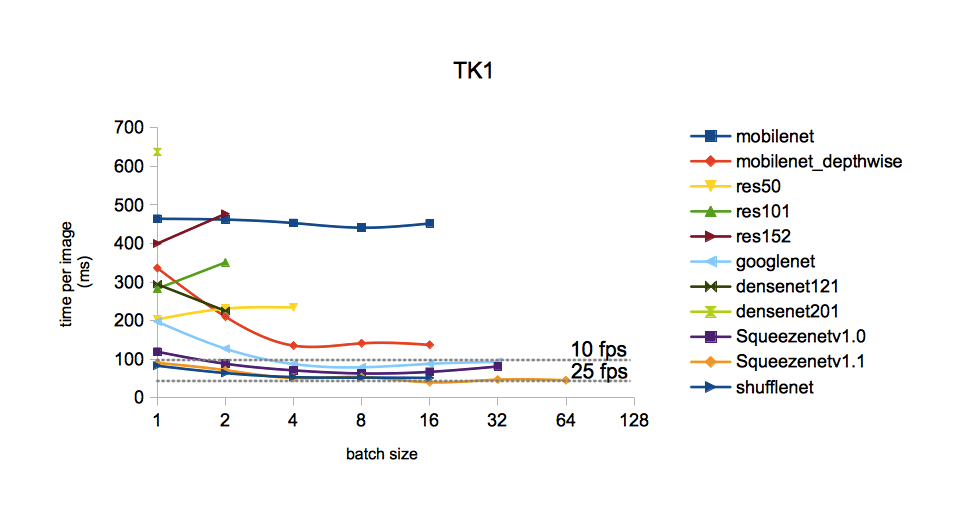
\includegraphics[width=.5\textwidth]{img/TK1_linear.png}\hfill
    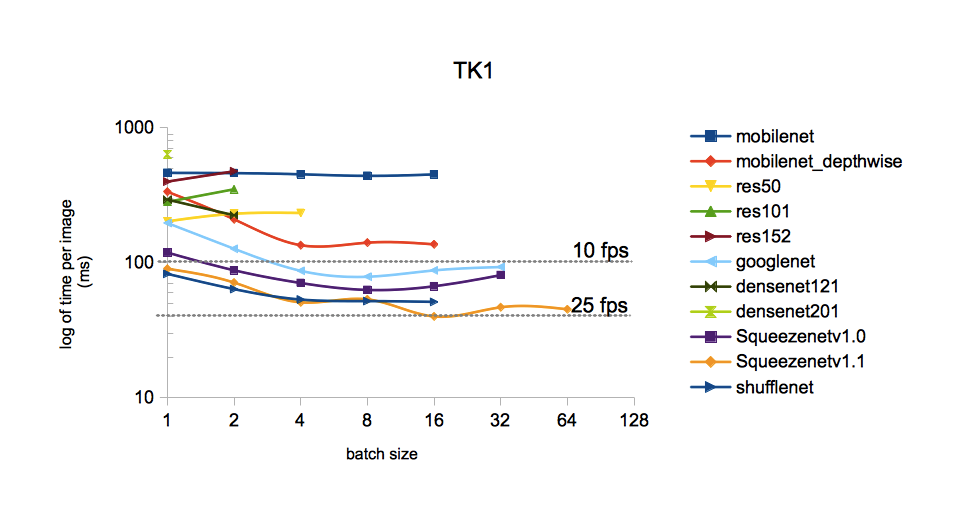
\includegraphics[width=.5\textwidth]{img/TK1_log.png}
    \caption{\textit{Benchmark} para la NVIDIA Jetson TK1. (Izquierda) tiempo de procesamiento lineal. (Derecha) tiempo de procesamiento en escala logarítmica.}
    \label{fig:ben_tk1}
\end{figure}

\begin{figure}[htp]
    \centering
    \captionsetup{justification=centering}
    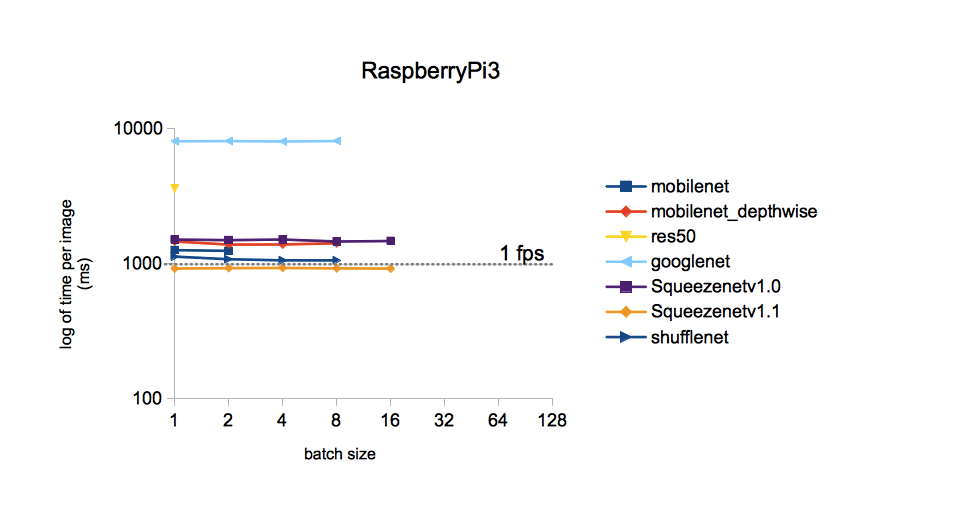
\includegraphics[width=.33\textwidth]{img/Raspi_log.png}\hfill
    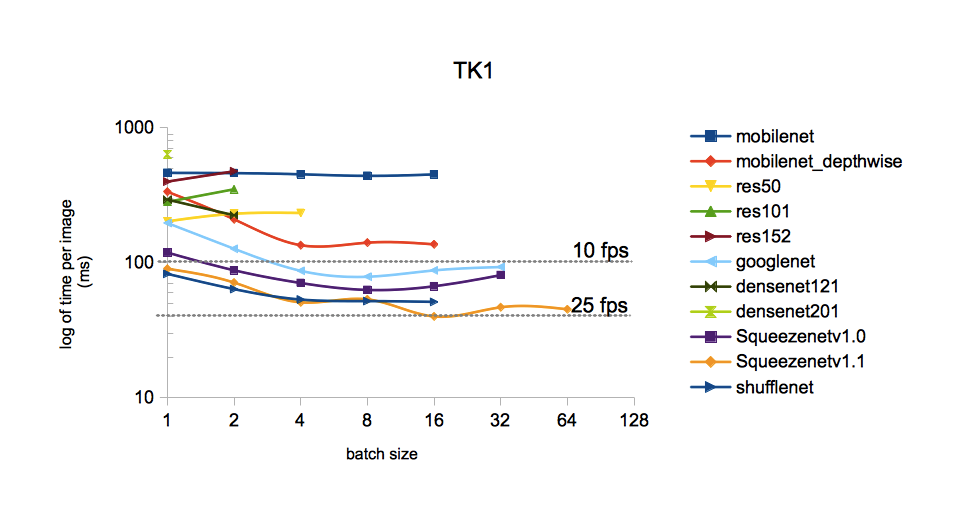
\includegraphics[width=.33\textwidth]{img/TK1_log.png}\hfill
    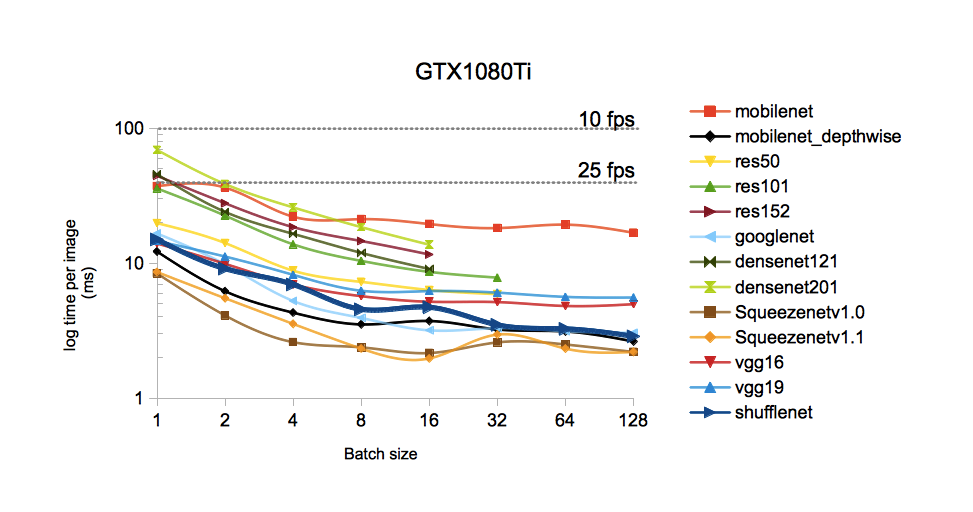
\includegraphics[width=.33\textwidth]{img/gtx1080_log.png}
    \caption{Comparativa entre RaspberryPi 3 (izquierda), Jetson TK1 (centro) y GTX 1080Ti (derecha).}
    \label{fig:ben_tk1_comp}
\end{figure}

\subsection{NVIDIA Jetson TX1}

En 2015, NVIDIA dio un paso adelante con su nueva placa para sistemas empotrados: la Jetson TX1 \cite{jetsontx1}. Esta placa de dimensiones aún más reducidas que su predecesora (50mm x 87mm) cuenta con un procesador ARM de 64-bits con 4 núcleos y una GPU con arquitectura Maxwell, ambos incluídos en el SoC (\textit{System-on-Chip}) Tegra X1, además de una memoria RAM de 4 GB con tecnología LPDDR4. Este módulo supuso un salto en capacidad de cómputo ya que el procesador dobla en poder al de la Jetson TK1 tanto en CPU como en GPU. Este salto en potencia, también se ve reflejado en el consumo, ya que a máxima carga, esta placa consume 15 W frente a los 12.5 W de la TK1.

En la Figura \ref{fig:ben_tx1} se reflejan los resultados de los \textit{benchmark} aplicados a esta placa. Comparando con los resultados de la placa TK1 (Figura \ref{fig:ben_tk1}), a simple vista se puede percibir que el salto en rendimiento y potencia es evidente. Mientras que la Jetson TK1, no es capaz de ofrecer tasas de refresco mayores que 25 fotogramas por segundo, la Jetson TX1 supera ese umbral en más de la mitad de las redes probadas. Y las redes más lentas como la \textit{densenet201} obtienen una mejora de rendimiento significativa en la placa TX1.
Comparada con la GTX 1080Ti (Figura \ref{fig:ben_gtx}), se puede ver que el rendimiento de la TX1 se acerca mucho a los resultados obtenidos por la 1080Ti. Hay que tener en cuenta que la placa Jetson TX1 cuenta con una tecnología propietaria de NVIDIA denominada Maxwell, cuyo chip implementa 256 núcleos CUDA; mientras que la GTX 1080Ti cuenta con una tecnología más avanzada, también propietaria de NVIDIA, denominada Pascal y cuyo chip implementa 3584 núcleos CUDA.

\begin{figure}[htp]
    \centering
    \captionsetup{justification=centering}
    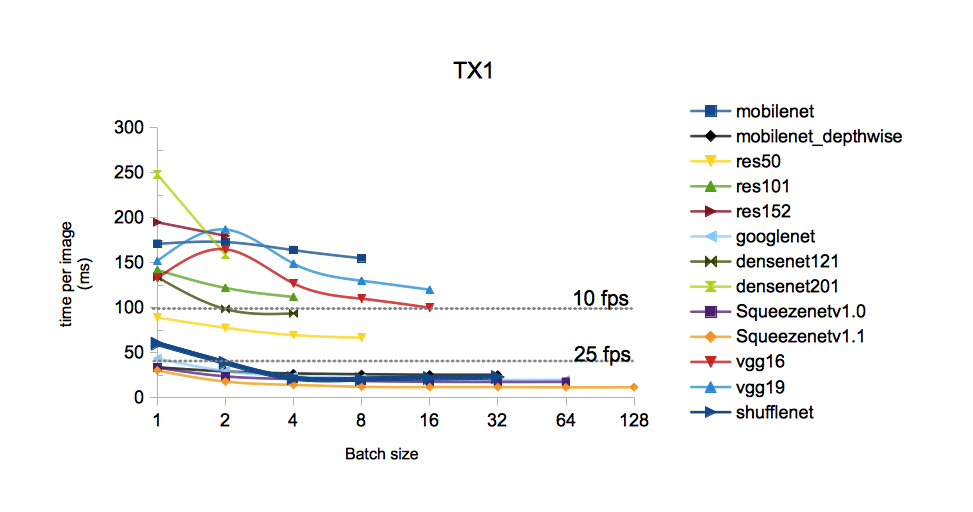
\includegraphics[width=.5\textwidth]{img/TX1_linear.png}\hfill
    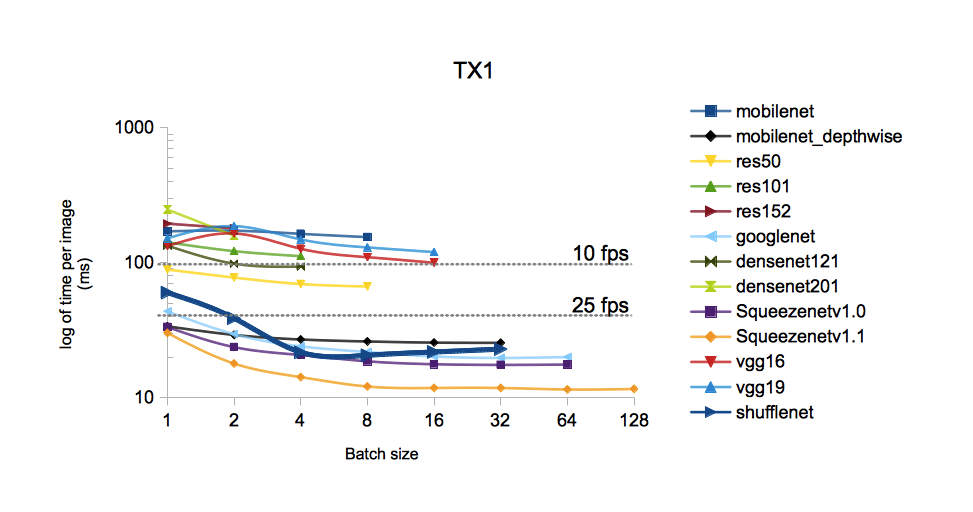
\includegraphics[width=.5\textwidth]{img/TX1_log.png}
    \caption{\textit{Benchmark} para la NVIDIA Jetson TX1. (Izquierda) tiempo de procesamiento lineal. (Derecha) tiempo de procesamiento en escala logarítmica.}
    \label{fig:ben_tx1}
\end{figure}

\begin{figure}[htp]
    \centering
    \captionsetup{justification=centering}
    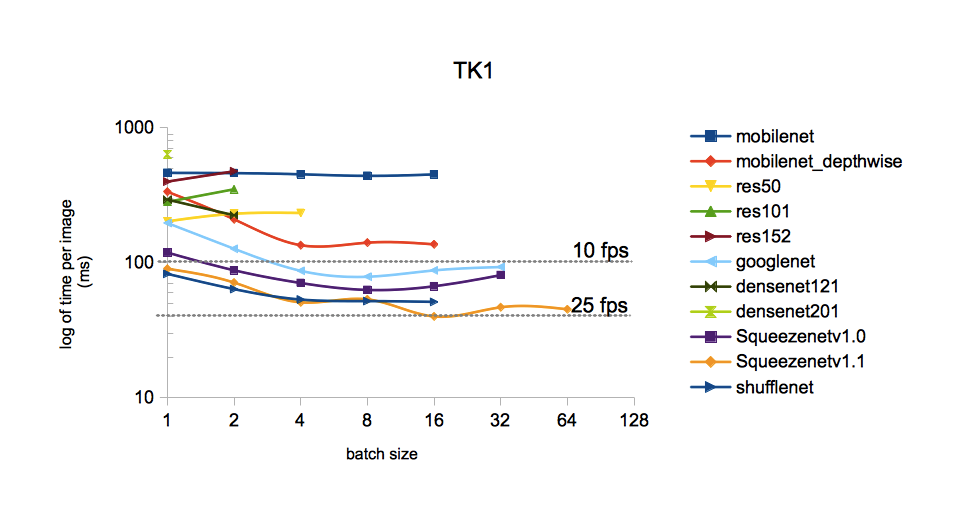
\includegraphics[width=.33\textwidth]{img/TK1_log.png}\hfill
    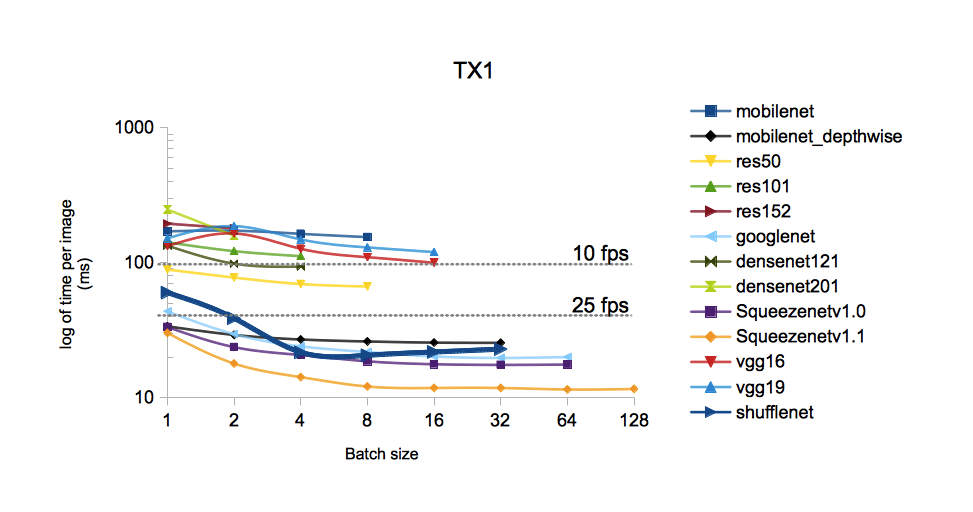
\includegraphics[width=.33\textwidth]{img/TX1_log.png}\hfill
    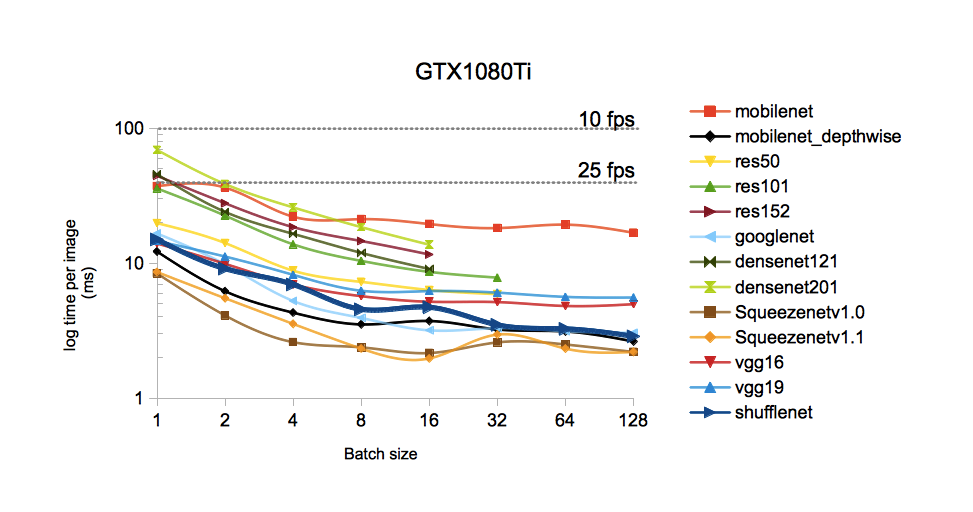
\includegraphics[width=.33\textwidth]{img/gtx1080_log.png}
    \caption{Comparativa entre Jetson TK1 (izquierda), Jetson TX1 (centro) y GTX 1080Ti (derecha). Escala logarítmica.}
    \label{fig:ben_tk1_comp_1080}
\end{figure}

\subsection{NVIDIA Jetson Nano}
\label{sec:jnano}

Este mismo año, en 2019 NVIDIA presentó sus nuevas placas de precio y prestaciones reducidas denominadas Jetson Nano \cite{jetsonnano}. Estas nueva placas siguen la línea de sus hermanas con un tamaño reducido (80mm x 100mm) pero con precio y prestaciones más bajos, aunque muy potentes y optimizadas para inteligencia artificial. Cuenta con un procesador ARM de 64-bits con 4 núcleos y una GPU basada en tecnología Maxwell (como sus hermana Jetson TX1) con la mitad de núcleos CUDA (128). Este módulo tiene dos modos de consumo: modo normal (5W) y carga máxima (10W), lo que lo hace el más liviano de toda la familia Jetson, además tiene un precio reducido con respecto al resto de placas de la familia. Cabe destacar, que el modo de consumo normal desactiva parte del hardware de la placa, ya que apaga 2 núcleos del procesador para ahorrar energía. No obstante, a máxima potencia, ofrece el máximo rendimiento hardware.

En la Figura \ref{fig:ben_nano} se tiene el resultado de los tests en la Jetson Nano. Comparado con su hermana la Jetson TX1 (Figura \ref{fig:ben_tx1}) se puede apreciar que el rendimiento es ligeramente más bajo debido a que tiene la mitad de núcleos en su CPU y su frecuencia de trabajo es más baja. No obstante, si se compara con la Jetson TK1 (Figura \ref{fig:ben_nano_comp} (izquierda)), se puede comprobar que la supera en rendimiento en todas las redes probadas. Hay que tener en cuenta, en este caso concreto, el consumo de ambas placas y el número de núcleos de GPU de ambas. Mientras que la Jetson TK1 cuenta con 192 núcleos CUDA en su GPU, la Jetson Nano cuenta con 128 núcleos. Además el consumo de la Jetson TK1 es más del doble que la Jetson Nano. Con todo eso, esta placa es superior a la TK1 en cuanto a ratio rendimiento/consumo. Para la misma red \textit{mobilenet}, la placa Nano bate en rendimiento a la TK1 acercándose a una tasa de fotogramas por segundo de 10, mientras que la TK1 permanece constante muy alejada de esos valores.

\begin{figure}[htp]
    \centering
    \captionsetup{justification=centering}
    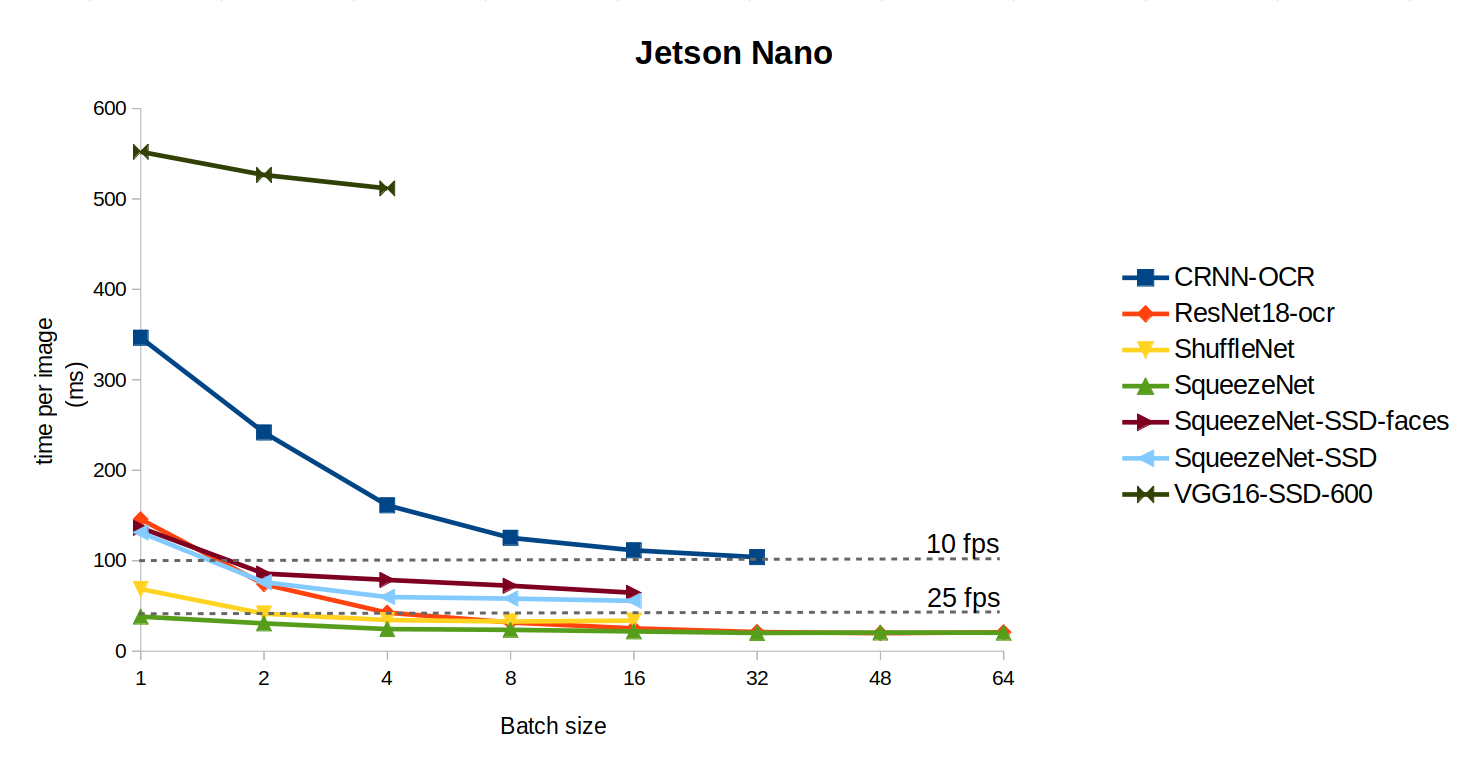
\includegraphics[width=.5\textwidth]{img/Jetson-nano-linear.png}\hfill
    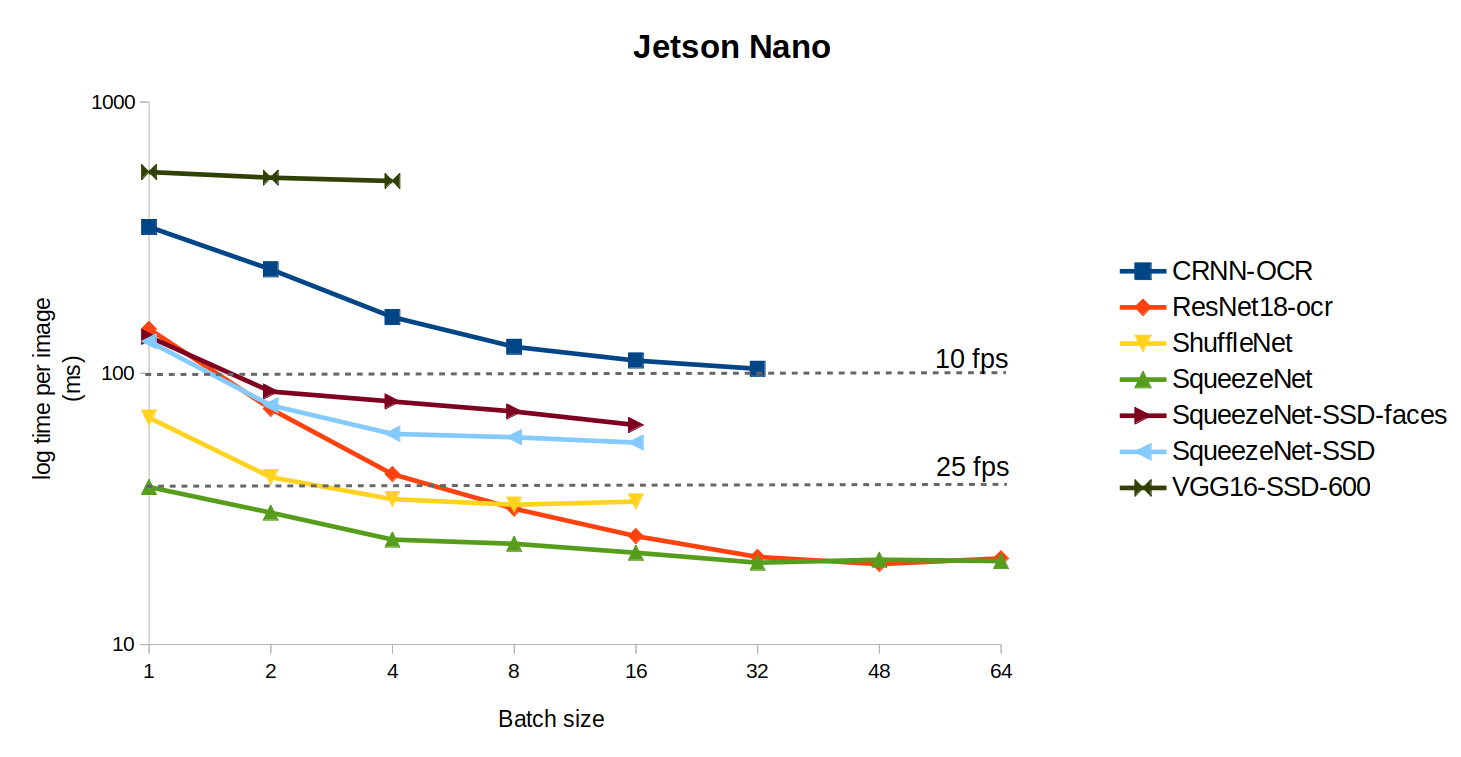
\includegraphics[width=.5\textwidth]{img/Jetson-nano-log.png}
    \caption{\textit{Benchmark} para la NVIDIA Jetson Nano. (Izquierda) tiempo de procesamiento lineal. (Derecha) tiempo de procesamiento en escala logarítmica.}
    \label{fig:ben_nano}
\end{figure}

\begin{figure}[htp]
    \centering
    \captionsetup{justification=centering}
    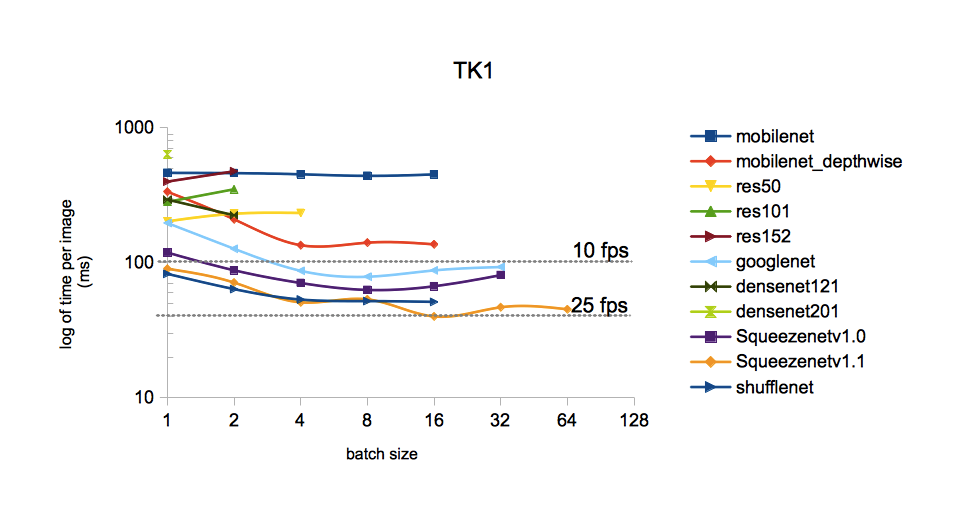
\includegraphics[width=.33\textwidth]{img/TK1_log.png}\hfill
    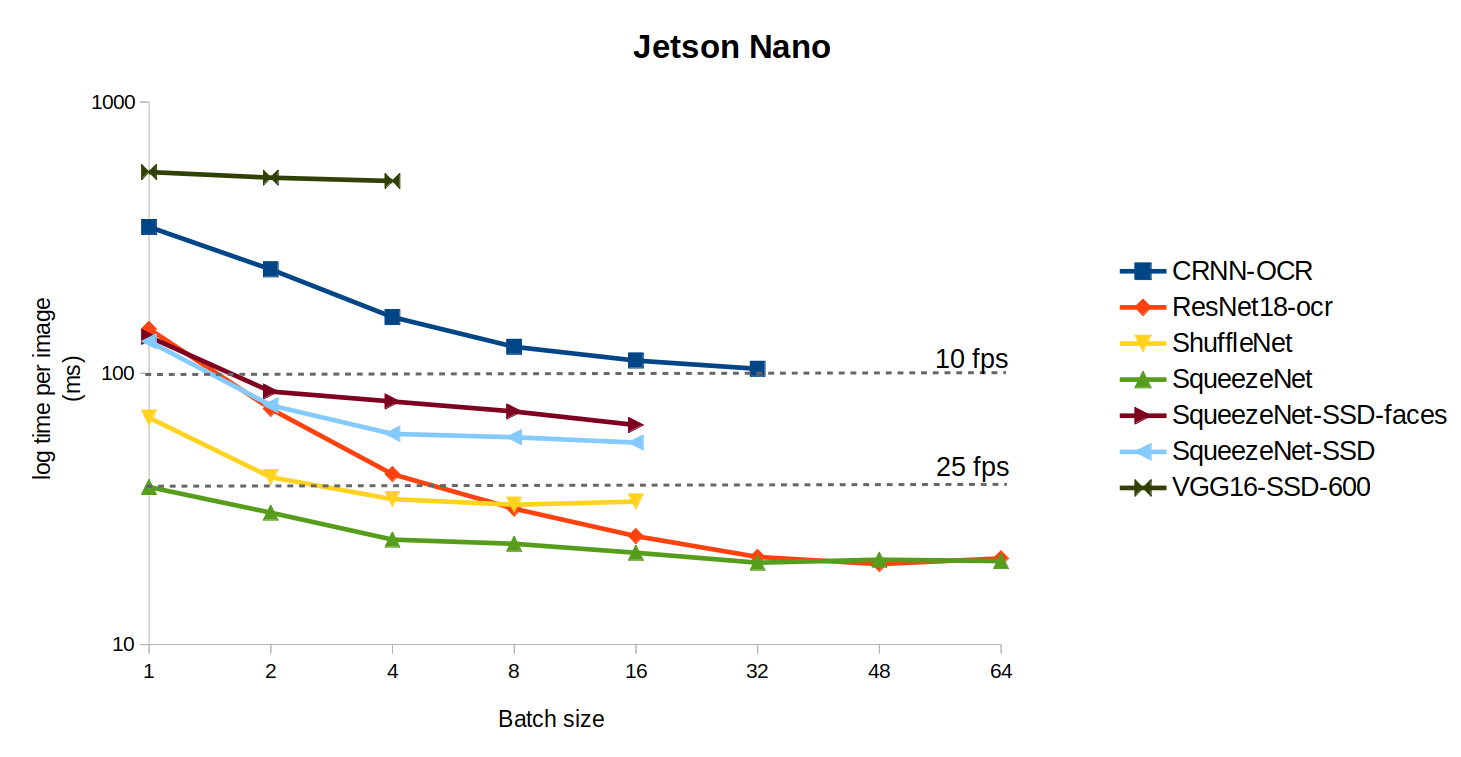
\includegraphics[width=.33\textwidth]{img/Jetson-nano-log.png}\hfill
    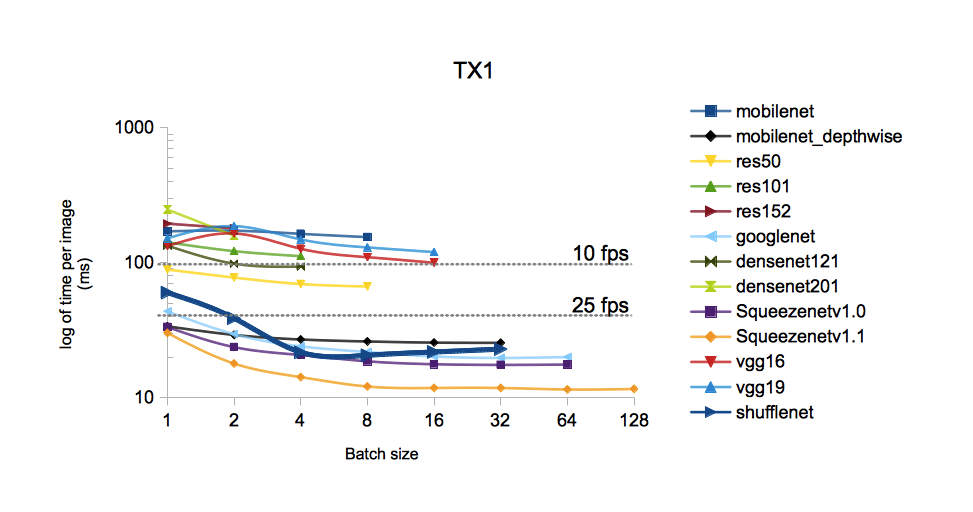
\includegraphics[width=.33\textwidth]{img/TX1_log.png}
    \caption{Comparativa entre Jetson TK1 (izquierda), Jetson Nano (centro) y Jetson TX1 (derecha). Escala logarítmica.}
    \label{fig:ben_nano_comp}
\end{figure}

\subsection{Google TPU \textit{Tensor Processing Unit}}

Google ha puesto a la venta su propio \textit{hardware} acelerador de cómputo, que hasta hace pocos meses no ofrecía. En su lugar, ofrecía servicios de computación en la nube como \textit{Google Colab}, en el que de forma gratuita se tiene acceso a un servidor para realizar cálculos en la nube con esta tecnología TPU que acelera en gran medida los tiempos de aprendizaje de las redes neuronales. La Figura \ref{fig:tpu} muestra una unidad de TPU de Google.

\begin{figure}[htp]
    \centering
    \captionsetup{justification=centering}
    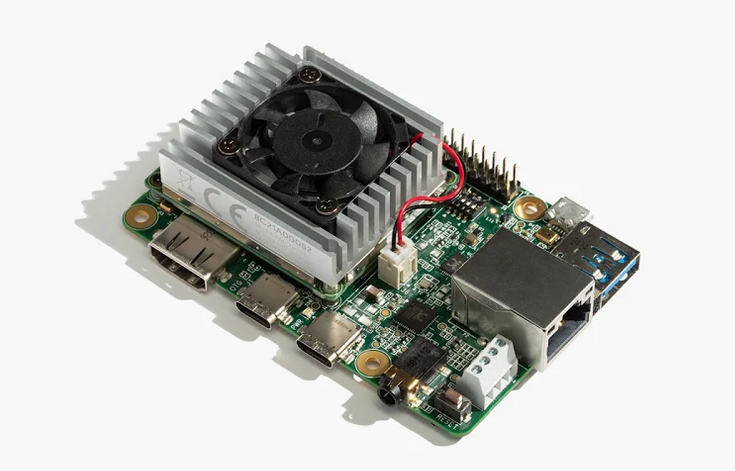
\includegraphics[width=.5\textwidth]{img/tpu.PNG}\hfill
    \caption{TPU de Google.}
    \label{fig:tpu}
\end{figure}

En 2018, Google presentó su propio \textit{hardware} acelerador de cómputo especializado en cálculo matricial y al que denominó TPU \cite{tpu}. Estas siglas, similares a las de GPU (\textit{Graphic Porcessing Unit}), vienen de \textit{Tensor Processing Unit} o Unidad de procesamiento de tensores. Un tensor no es más que una matriz multidimensional. La ventaja de las TPU es que pueden realizar cálculos en paralelo a una gran velocidad y, dado su carácter optimizado para el cálculo matricial (álgebra lineal), son ideales para la ejecución algoritmos de aprendizaje automático para visión artificial al ser la información que procesan estas redes matrices (imágenes).

No obstante, esta tecnología está pensada para ser utilizada en determinados ámbitos de trabajo concretos, de tal forma que en cómputo de carácter más general es más recomendable utilizar CPU o GPU.

\begin{itemize}
    \item CPU. Recomendado para realizar prototipos rápidos que requieran mucha flexibilidad. Entrenar modelos sencillos, pequeños y limitados.
    \item GPU. Modelos con un número notable de operaciones y con tamaños de lote grandes.
    \item TPU. Modelos de cómputo de matrices, con amplio tiempo de entrenamiento. Modelos muy grandes.
\end{itemize}

\begin{comment}
\section{Conclusiones}

Se han visto las tecnologías más punteras en cuanto a procesamiento de datos con redes neuronales, utilizando conjuntos de datos obtenidos para resolver el problema de la conducción autónoma. Además, se han visto las últimas tendencias en cuanto a \textit{hardware} acelerador de cómputo, con propuestas de diferentes empresas privadas que están a la cabeza en el sector tecnológico. Los algoritmos que se han explicado aquí son casos de éxito de los mismos en problemas de conducción autónoma, por lo que este TFM propone la ejecución de estos algoritmos en sistemas empotrados muy eficientes, de forma que se solvente el problema de cómputo de las redes neuronales, que necesitan hardware muy potente, y, por ende, muchos recursos en cuanto a alimentación de ese \textit{hardware} y espacio físico.

Las tecnologías explicadas en este estado del arte, intentarán aplicarse en este proyecto en mayor o menor medida, en cuanto a las capacidades y disponibilidad de \textit{hardware} en el momento de su desarrollo.
\end{comment}